% Set up the document
\documentclass{article}

% Page size
\usepackage[
    letterpaper,]{geometry}

% Lines between paragraphs
\setlength{\parskip}{\baselineskip}
\setlength{\parindent}{0pt}

% Math
\usepackage{mathtools}
\usepackage{amssymb}
\usepackage{amsthm}
\usepackage{commath}

\DeclarePairedDelimiter\ceil{\lceil}{\rceil}
\DeclarePairedDelimiter\floor{\lfloor}{\rfloor}

% Number sets
\newcommand{\C}{\mathbb{C}}
\newcommand{\T}{\mathbb{T}}
\newcommand{\N}{\mathbb{N}}
\newcommand{\Q}{\mathbb{Q}}
\newcommand{\R}{\mathbb{R}}
\newcommand{\Z}{\mathbb{Z}}

% Links
\usepackage{hyperref}

% Page numbers at top right
\usepackage{fancyhdr}
\pagestyle{fancy}
\fancyhf{}
\fancyhead[R]{\thepage}
\renewcommand\headrulewidth{0pt}

% Graphics
\usepackage{float}
\usepackage{graphicx}
\graphicspath{ {./img/} }

% MATLAB stuff
\usepackage[numbered,framed]{matlab-prettifier}
\lstset{
  style              = Matlab-editor,
  mlshowsectionrules = true,
}

\begin{document}

\textbf{MATH 419 homework 2} \\
\textbf{Matt Wiens \#301294492} \\
\textbf{2020-06-16}

3.1. Create a MATLAB script to reproduce Figure 3.1 (from the course
  textbook). Experiment with other values of $N$. Describe what you see.
  Near the jump discontinuity you will see an overshoot that remains
  large as $N$ increases. This is the Gibbs phenomenon. Repeat the
  exercise for the square wave function that arises as the periodic
  extension of the following step function $g(\theta)$:
%
\begin{equation*}
    g(\theta) =
    \begin{cases}
        1,&\theta \in [0, \pi) \\
        -1,&\theta \in [- \pi, 0)
    \end{cases}
    .
\end{equation*}

\textit{Solution.} First let's sort out the partial Fourier sums for
both the sawtooth function $f$ and the square wave function $g$. From
the textbook we have that the partial Fourier sums for the sawtooth
function are given by
%
\begin{equation*}
    S_N f = 2 \sum_{n = 1}^N \frac{(-1)^{n + 1}}{n} \sin(n \theta)
    .
\end{equation*}
%
For the square wave function the Fourier coefficients are given by
%
\begin{align*}
    \widehat{g}(n)
        &\coloneqq \frac{1}{2 \pi} \int_{-\pi}^\pi g(\theta) e^{-i n \theta} \dif \theta \\
        &= \frac{1}{2 \pi}
            \del{
                \int_{-\pi}^0 (-1) e^{-i n \theta} \dif \theta
                +
                \int_0^{\pi} e^{-i n \theta} \dif \theta
            } \\
        &= \frac{i}{2 n \pi}
            \del{
                (e^{i n \pi} - 1)
                +
                (e^{-i n \pi} - 1)
            } \\
        &= \frac{i}{n \pi} (\cos(n \pi) - 1) \\
        &= \frac{i}{n \pi} ((-1)^{n} - 1)
        .
\end{align*}
%
Hence the partial Fourier sums are given by
%
\begin{align*}
    S_N g &= \sum_{n = - N}^N \frac{i}{n \pi} ((-1)^{n} - 1) e^{i n \theta} \\
          &= \frac{2}{\pi} \sum_{n = 1}^N \frac{1}{n} (1 - (-1)^{n}) \sin(n \theta)
          .
\end{align*}
%
Note that we dropped the $n = 0$ term because it is zero (as are all
even terms). We could simplify further, but for the purposes of this
question, the above expression does the job.

In Figure~\ref{fig:3-1-a} partial Fourier sums for various values of $N$
are plotted along with the line $y = \pi$ (which is the maximum value
the sawtooth function takes). We see for sufficiently large values of
$N$ (looks like it's about $N = 3$ here) we get oscillatory behaviour
close to the jump discontinuities, and that it consistently overshoots
the maximum value of the sawtooth function at these points.

In Figure~\ref{fig:3-1-b} partial Fourier sums for various values of $N$
are plotted along with the line $y = 1$ (which is the maximum value the
square wave function takes). Again we see the same behaviour as with the
sawtooth function. However, it takes longer for the partial Fourier sums
(in terms of larger values of $N$) to be smooth in-between jump
discontinuities for the square wave function than for the sawtooth
function.

The code used to produce both Figure~\ref{fig:3-1-a} and~\ref{fig:3-1-b} is
contained in Listing~\ref{lst:1}.


\newpage

\begin{figure}[hbtp]
    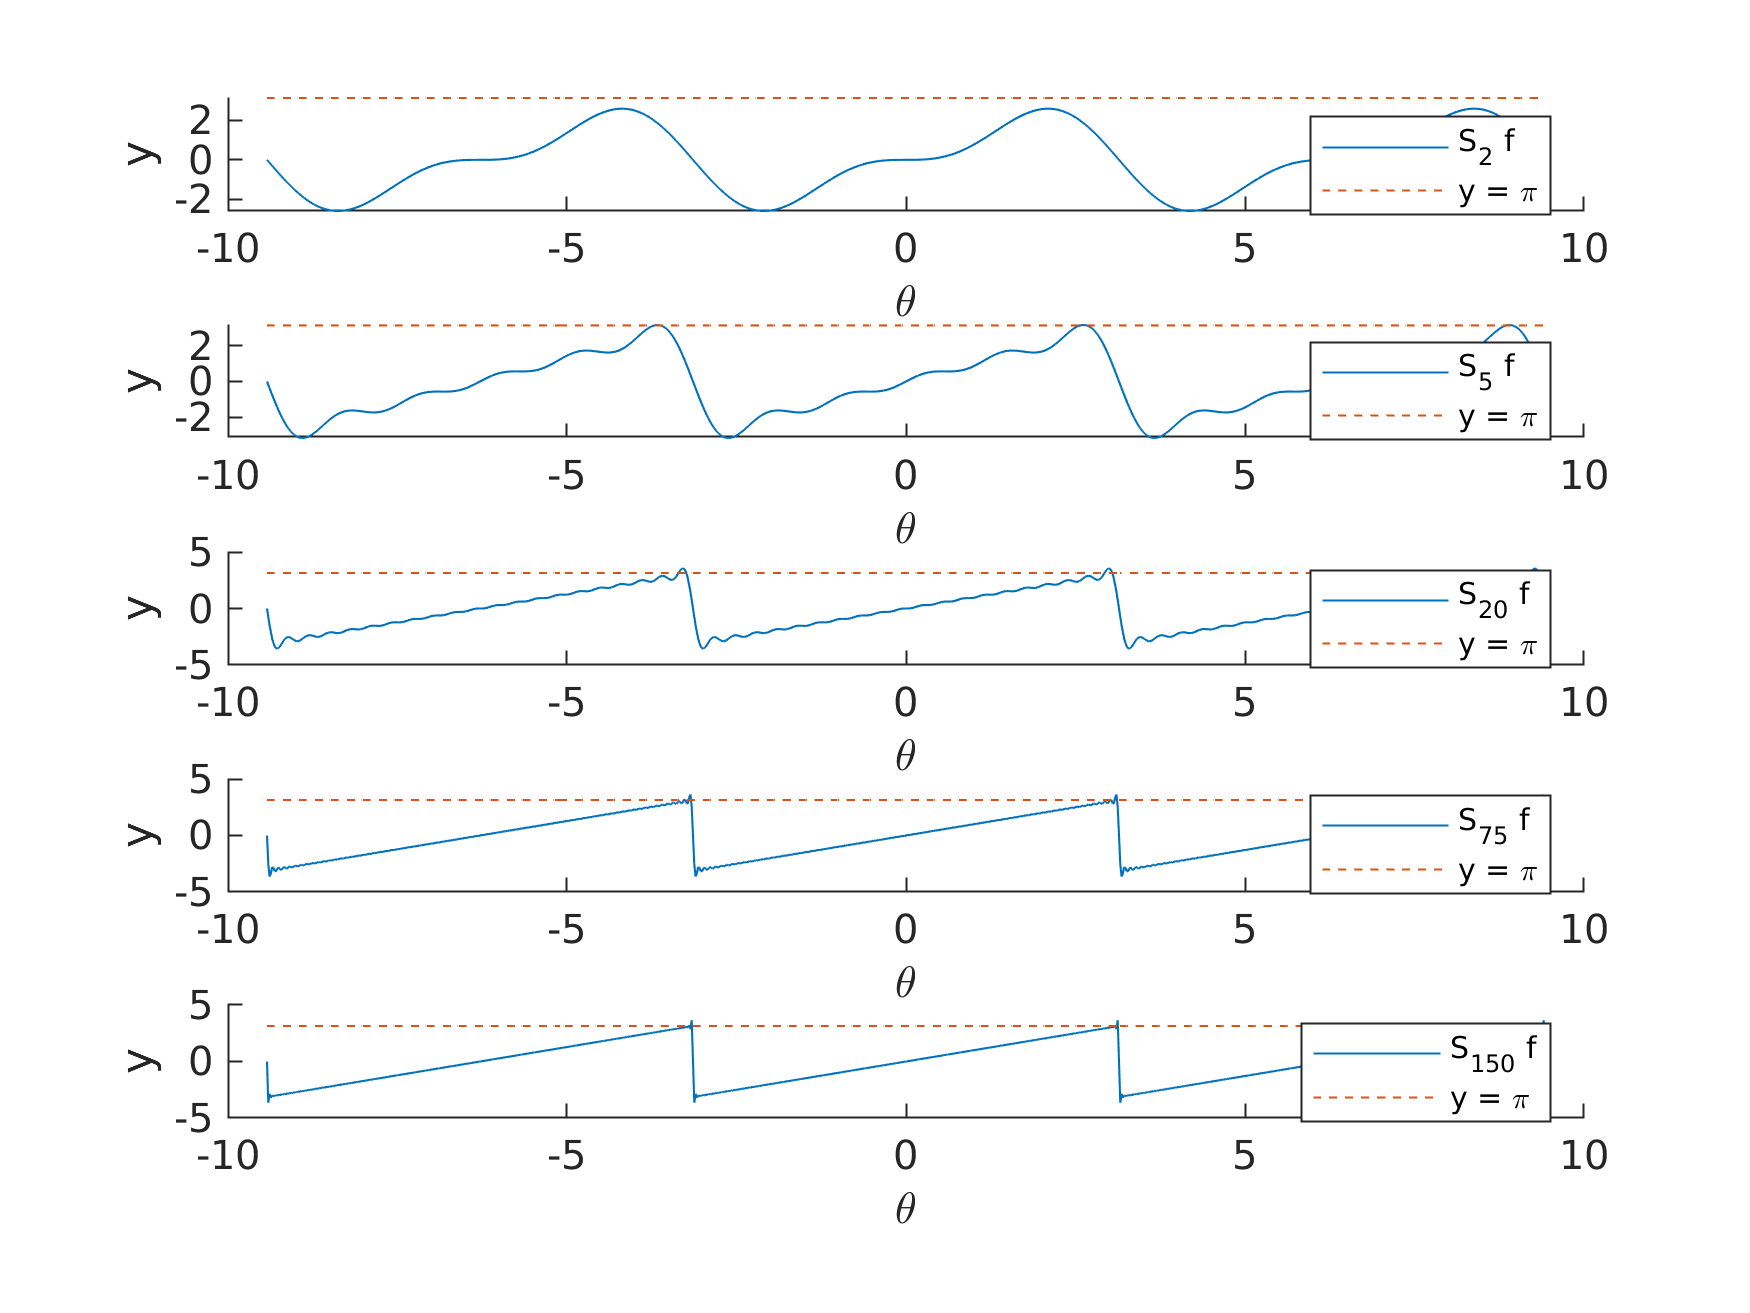
\includegraphics[width=\textwidth]{q31a}
    \centering
    \caption{Partial Fourier sums for the sawtooth function}
    \label{fig:3-1-a}
\end{figure}

\newpage

\begin{figure}[hbtp]
    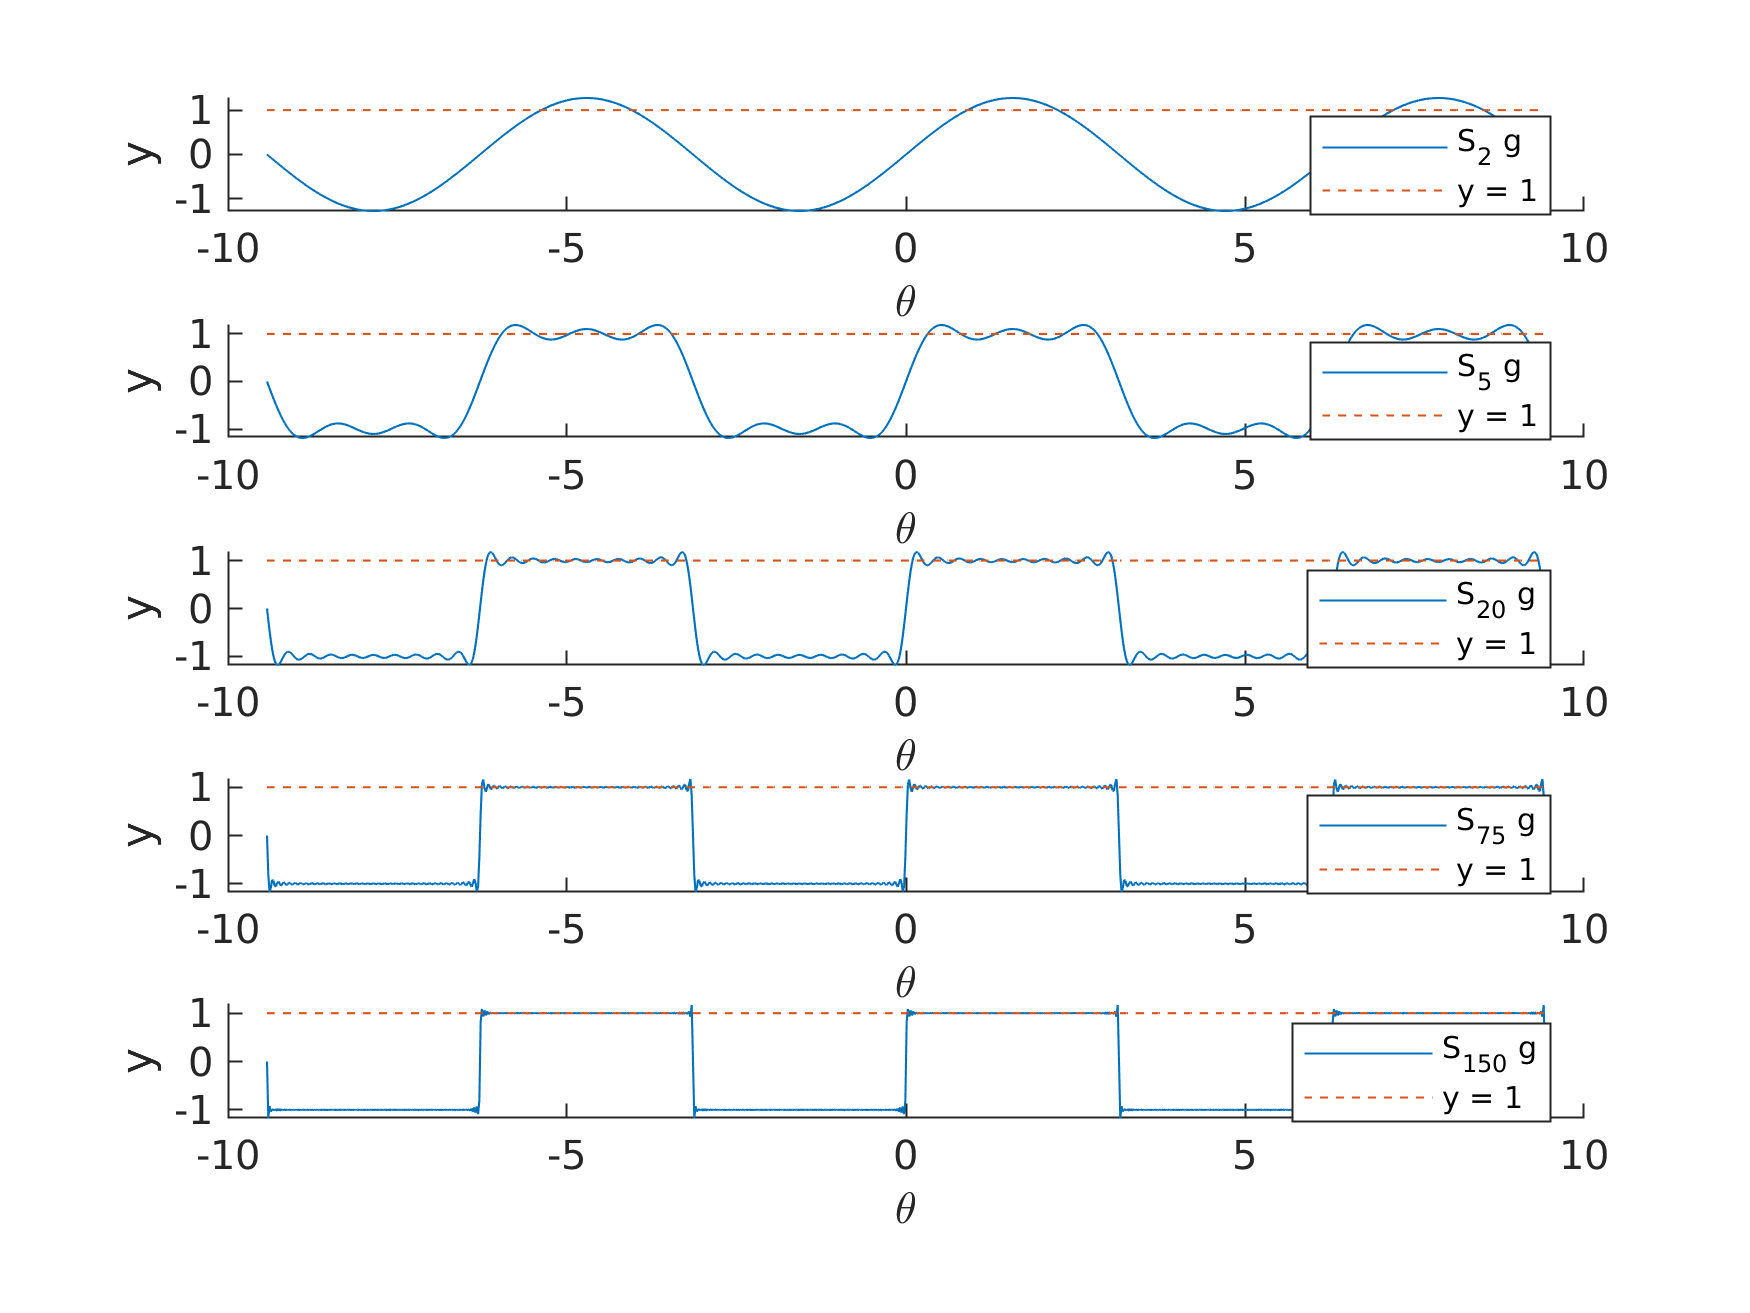
\includegraphics[width=\textwidth]{q31b}
    \centering
    \caption{Partial Fourier sums for the square wave function}
    \label{fig:3-1-b}
\end{figure}

\newpage

\lstinputlisting[caption={Code to generate plots},captionpos=b,label={lst:1}]{./code/q31.m}

\newpage

3.11. Prove Lemma 3.10. Give an example to show that if the sequence of
  averages converges, that does not imply that the original sequence
  converges.

\textit{Solution.}
Suppose the sequence $\cbr{a_n}$ converges to some limit $a$. Define
%
\begin{equation*}
    \bar{a}_n = \frac{1}{n} \sum_{k = 1}^n a_k
    .
\end{equation*}
%
We want to show that $\bar{a}_n$ also converges to $a$.

Fix $\epsilon > 0$. Choose $N_1 > 0$ such that for all $n > N_1$ we
have $\envert{a_n - a} < \frac{\epsilon}{2}$. We start by expressing
$\envert{\bar{a}_n - a}$  (where $n > N_1$) as
%
\begin{align*}
    \envert{\bar{a}_n - a}
        &= \envert{\frac{1}{n} \sum_{k = 1}^{n} a_n - a } \\
        &= \envert{\frac{1}{n} \sum_{k = 1}^{n} (a_n - a)} \\
        &= \envert{
            \frac{1}{n} \sum_{k = 1}^{N_1} (a_n - a)
            +
            \frac{1}{n} \sum_{k = N_1 + 1}^{n} (a_n - a)
        }
        .
\end{align*}
%
Applying the triangle inequality we have
%
\begin{equation}
    \envert{\bar{a}_n - a}
        \leq
            \frac{1}{n} \sum_{k = 1}^{N_1} \envert{a_n - a}
            +
            \frac{1}{n} \sum_{k = N_1 + 1}^{n} \envert{a_n - a}
        \label{eq:311a}
        .
\end{equation}
%
Since $\cbr{a_n}$ is bounded (because it is convergent), there exists
$M \geq 0$ such that $\envert{a_n - a} \leq M$ for all $n \in \N$. Let
$N_2 > 0$ be such that
%
\begin{equation*}
    \frac{N_1 M}{N_2} < \frac{\epsilon}{2}
    .
\end{equation*}
%
Now, letting $N = \max \cbr{N_1 + 1, N_2}$ and setting $n \geq N$, we
can bound the first term on the left hand side of~\eqref{eq:311a} as
%
\begin{equation*}
    \frac{1}{n} \sum_{k = 1}^{N_1} \envert{a_n - a}
    \leq \frac{N_1 M}{n}
    \leq \frac{N_1 M}{N_2}
    < \frac{\epsilon}{2}
    ,
\end{equation*}
%
and for the second term we have
%
\begin{equation*}
    \frac{1}{n} \sum_{k = N_1 + 1}^{n} \envert{a_n - a}
    < \frac{1}{n} \sum_{k = N_1 + 1}^{n} \frac{\epsilon}{2}
    = \frac{n - N_1}{n} \frac{\epsilon}{2}
    < \frac{\epsilon}{2}
    .
\end{equation*}
%
Hence for $n \geq N$ we have
%
\begin{equation*}
    \envert{\bar{a}_n - a}
        \leq
            \frac{1}{n} \sum_{k = 1}^{N_1} \envert{a_n - a}
            +
            \frac{1}{n} \sum_{k = N_1 + 1}^{n} \envert{a_n - a}
        < \frac{\epsilon}{2} + \frac{\epsilon}{2} = \epsilon
        .
\end{equation*}
%
This shows that $\cbr{\bar{a}_n}$ converges to $a$, which concludes the
proof of Lemma 3.10.

We are now asked to show a counterexample for when a sequence of
averages converges but the original sequence does not.
Let $\cbr{a_n}$ be the sequence with elements $a_n = (-1)^n$.
Clearly this sequence fails to converge; however the sequence of averages
$\cbr{\bar{a}_n}$ with elements
%
\begin{equation*}
    \bar{a}_n =
        \begin{dcases}
            -\frac{1}{n},& \text{$n$ is odd} \\
            0,& \text{otherwise}
        \end{dcases}
\end{equation*}
%
converges to $0$.

\newpage

3.18. Deduce Corollary 3.17 from Theorem 3.16.

\textit{Solution.}
Let $f: \T \to \C$ be a $2\pi$-periodic integrable function.
Suppose that
%
\begin{equation*}
    |\widehat{f}(n)| \leq A |n|^{-k}
\end{equation*}
%
for $k \geq 2$ and $n \neq 0$, where $A$ is a positive constant. We want
to show that $f \in C^l(\T)$, where $l = k - 2$ if $k$ is an integer and
$l = \floor{k} - 1$ otherwise.

Let $l$ be as described above. Given our assumption on the Fourier
coefficients, we have that
%
\begin{align*}
    \sum_{n \in \Z} |\widehat{f}(n)| |n|^l
        &\leq \widehat{f}(0) \cdot 0^l + \sum_{\substack{n \in \Z \\ n \neq 0}} A |n|^{-k} |n|^l \\
        &= \widehat{f}(0) \cdot 0^l + 2 A \sum_{n = 1}^\infty n^{l - k}
        .
\end{align*}
%
If $k \in \Z$ then we have that $l - k = (k - 2) - k = -2 < -1$ and if
$k \not\in \Z$ we have $l - k = (\floor{k} - 1) - k) < - 1$.
In any case we have $l - k < -1$. Thus
%
\begin{equation*}
    \sum_{n = 1}^\infty n^{l - k} < \infty
\end{equation*}
%
and so
%
\begin{equation*}
    \sum_{n \in \Z} |\widehat{f}(n)| |n|^l < \infty
    .
\end{equation*}
%
Since $l \geq 0$, we can apply Theorem 3.16 to conclude that
$f \in C^l(\T)$.

\newpage

3.21. Show that if $f$ is continuous and $2\pi$-periodic, then it is
  uniformly continuous on $[-\pi, 2 \pi]$. Moreover, the functions
  $g_n(\theta) \coloneqq |f(\theta) - f(\theta + \pi/n)|$ converge
  uniformly to zero.

\textit{Solution.}
Since $f$ is continuous and $[-\pi, 2\pi]$ is a closed bounded interval,
we automatically have that $f$ is uniformly continuous on $[-\pi, 2\pi]$.

Fix any $\epsilon > 0$. Then we have that there exists $\delta > 0$ such
that for all $\theta_1, \theta_2 \in [-\pi, 2 \pi]$,
$|\theta_1 - \theta_2| < \delta$ implies $|f(\theta_1) - f(\theta_2)| < \epsilon$.

Fix any $\theta \in [-\pi, \pi]$ and let
$\theta_1 = \theta, \theta_2 = \theta + \pi / n$ for $n \in \N$. Note
that $\theta_1, \theta_2 \in [-\pi, 2 \pi]$. Then we have that if
%
\begin{equation*}
    |\theta_1 - \theta_2| = \envert{-\frac{\pi}{n}} = \frac{\pi}{n} < \delta
    ;
\end{equation*}
%
that is, if $n > \pi / \delta$, then
$|f(\theta) - f(\theta + \pi/n)| < \epsilon$.

Hence if we let $N = \ceil{\pi / \delta} + 1$, then for all $n \geq N$,
$g_n(\theta) < \epsilon$ for all $\theta \in [-\pi, \pi]$. Thus the
sequence of functions $\cbr{g_n(\theta)}$ converges uniformly to zero.

\newpage

3.22. A function $f: \T \to \C$ is called Lipchitz if there is a constant $k$ such that
$|f(\theta_1) - f(\theta_2)| \leq k |\theta_1 - \theta_2|$ for all
$\theta_1, \theta_2 \in \T$. Show that if $f$ is Lipchitz, then
%
\begin{equation*}
    |\widehat{f}(n)| \leq \frac{C}{n}
\end{equation*}
%
for some constant $C$ independent of $n \in \Z$.

\textit{Solution.}
Suppose the function $f$ is Lipchitz. We also need to assume that $n
\neq 0$ (the question doesn't make much sense otherwise). We'll use
several tricks demonstrated in lectures to get bounds on the Fourier
coefficients of $f$. The first trick we'll use is multiplying by $1 =
(-1) e^{i \pi}$, using a substitution, and then making use of
$2\pi$-periodicity to simplify the limits of integration:
%
\begin{align*}
    \widehat{f}(n)
        &\coloneqq \frac{1}{2 \pi} \int_{-\pi}^\pi f(\theta) e^{-i n \theta} \dif \theta \\
        &= \frac{1}{2 \pi} \int_{-\pi}^\pi f(\theta) e^{-i n \theta} (-1) e^{i \pi} \dif \theta \\
        &= - \frac{1}{2 \pi} \int_{-\pi}^\pi f(\theta) e^{-i n \del{\theta - \frac{\pi}{n}}} \dif \theta \\
        &= - \frac{1}{2 \pi} \int_{-\pi - \frac{2 \pi}{n}}^{\pi - \frac{2 \pi}{n}} f\del[2]{x + \frac{\pi}{n}} e^{-i n x} \dif x \\
        &= - \frac{1}{2 \pi} \int_{-\pi}^{\pi} f\del[2]{\theta + \frac{\pi}{n}} e^{-i n \theta} \dif \theta
        .
\end{align*}
%
Note that on the fourth line we made the substitution
$x = \theta - \pi / n$, and on the fifth line we simply used $\theta$
instead of $x$ as the dummy variable. The next trick we'll use is to
average the first and fifth lines to write
%
\begin{equation*}
    \widehat{f}(n) = \frac{1}{4 \pi} \int_{-\pi}^{\pi}
        \del{f(\theta) - f\del[2]{\theta + \frac{\pi}{n}}}
        e^{-i n \theta}
        \dif \theta
\end{equation*}
%
Taking the absolute value of this expression and applying the triangle
inequality, we get
%
\begin{align*}
    |\widehat{f}(n)|
        &\leq \frac{1}{4 \pi} \int_{-\pi}^{\pi}
        \envert[3]{f(\theta) - f\del[2]{\theta + \frac{\pi}{n}}}
        \envert[1]{e^{-i n \theta}}
        \dif \theta
        \\
        &= \frac{1}{4 \pi} \int_{-\pi}^{\pi}
        \envert[3]{f(\theta) - f\del[2]{\theta + \frac{\pi}{n}}}
        \dif \theta
    .
\end{align*}
%
Now we can use that $f$ is Lipchitz, and so for some constant $k$ we have
%
\begin{equation*}
    |\widehat{f}(n)|
        \leq \frac{1}{4 \pi} \int_{-\pi}^{\pi}
        \envert[3]{f(\theta) - f\del[2]{\theta + \frac{\pi}{n}}}
        \dif \theta
        \leq \frac{1}{4 \pi} \int_{-\pi}^{\pi}
        k \frac{\pi}{n}
        \dif \theta
        = \frac{\pi k}{2 n}
    .
\end{equation*}
%
Hence taking $C = \pi k / 2$ we have that
%
\begin{equation*}
    |\widehat{f}(n)| \leq \frac{C}{n}
    .
\end{equation*}

\newpage

3.26. Show that if $f$ is an integrable even function, then $\hat{f}(n)
  = \hat{f}(-n)$ for all $n \in \Z$. This means that the corresponding
  Fourier series is a purely cosine series expansion.

\textit{Solution.}
Suppose that $f$ is an integrable even function. Then we have that,
using the fact that $f(\theta) = f(-\theta)$ and the substitution
$x = - \theta$,
%
\begin{align*}
    \widehat{f}(n)
        &\coloneqq \frac{1}{2 \pi} \int_{-\pi}^\pi f(\theta) e^{-i n \theta} \dif \theta \\
        &= \frac{1}{2 \pi} \int_{-\pi}^\pi f(-\theta) e^{-i n \theta} \dif \theta \\
        &= - \frac{1}{2 \pi} \int_{\pi}^{-\pi} f(x) e^{i n x} \dif x \\
        &= \frac{1}{2 \pi} \int_{-\pi}^{\pi} f(x) e^{-i (-n) x} \dif x \\
        &= \widehat{f}(-n)
        .
\end{align*}

\end{document}
